%======================================================================
%===  dtuposter - a class to make posters tha comply with the DTU CI
%
% Written and maintained in 2011-2014 
% by Jorrit Wronski (jowr@mek.dtu.dk)
%
%
%==========================================
%===  details and poster setup
\documentclass[
%    ,title     = {{Title test}}
%    author    = {{Soeren Winkel Holm}}
%    ,subject   = {{This is the subject of my work}}
%    ,bgcolor   = dtulightgreen
%    ,highlight = dtuyellow
%    ,toplogo   = {{tex_dtu_aqua_b_uk}}
%    ,botlogo   = {{tex_dtu_bibliotek_b_uk}}
%    ,papersize = {{a0paper}}
%    ,colcount  = {{1column}}
%    ,longtitle
%    ,largecaption
%    ,draft
%    ,nocrop
%    ,english        % language
%    ,fleqn          % equations on the left
]{dtuposter}
%
%
%======================================================================
%===  Continue with packages
\usepackage[T1]{fontenc}        % special characters
%
%\usepackage[ansinew]{inputenc}  % Windows
%\usepackage[applemac]{inputenc} % MacOS
\usepackage[utf8]{inputenc}    % Unicode, Linux

%
% 
%======================================================================
%=== Font definitions, DTU recommends Arial for posters
%\usepackage{cmbright}
%\usepackage{arevmath}
%\usepackage[scaled]{uarial} %Arial clone, set as default sf font - use "ua1" for direct access
%\usepackage{uarial} %Arial clone, set as default sf font - use "ua1" for direct access
%\usepackage[typeface=default,
%            sanstypeface=urwarial,
%            mathtypeface=arevmath
%           ]{typeface}
\renewcommand{\familydefault}{\sfdefault}
\usepackage{enumitem}
\setlist{nosep,leftmargin=*}
%
% 
%======================================================================
%=== Other useful packages
\usepackage{booktabs}

\usepackage{float}
\usepackage[caption = false]{subfig}
%======================================================================
%=== The actual content starts here
\begin{document}
%
%
%======================================================================
%===  Make header for poster (title and authors)
\begin{dtuposterhead} %
\dtuposterauthor{Mads Andersen, Oskar Wiese, Anders Henriksen, Søren Holm, Asger Schultz}
\dtuposteraffil{DTU Compute}
\dtuposteraffil{\texttt{\{s173934, s183917, s183904, s183911, s183912\}@student.dtu.dk}}
\end{dtuposterhead}
%
%
%======================================================================
%===  ... and the rest of the content
\begin{dtupostercontent}
\section{Weeds, Crops and Dirt}
 
\section{The Data: Brazilian Sugar Fields}
The data used in this project is one drone image of a field, which is illustrated as the following.
\begin{figure}
\centering
\includegraphics[width=.7\linewidth]{raw-min}
\end{figure}


\section{Our SegNet: 1152 Feature Maps}

%%Model af netværket 
%%Encoder-Decoder
%% "Skip connections"" + Adam 

\begin{figure}
	\centering
	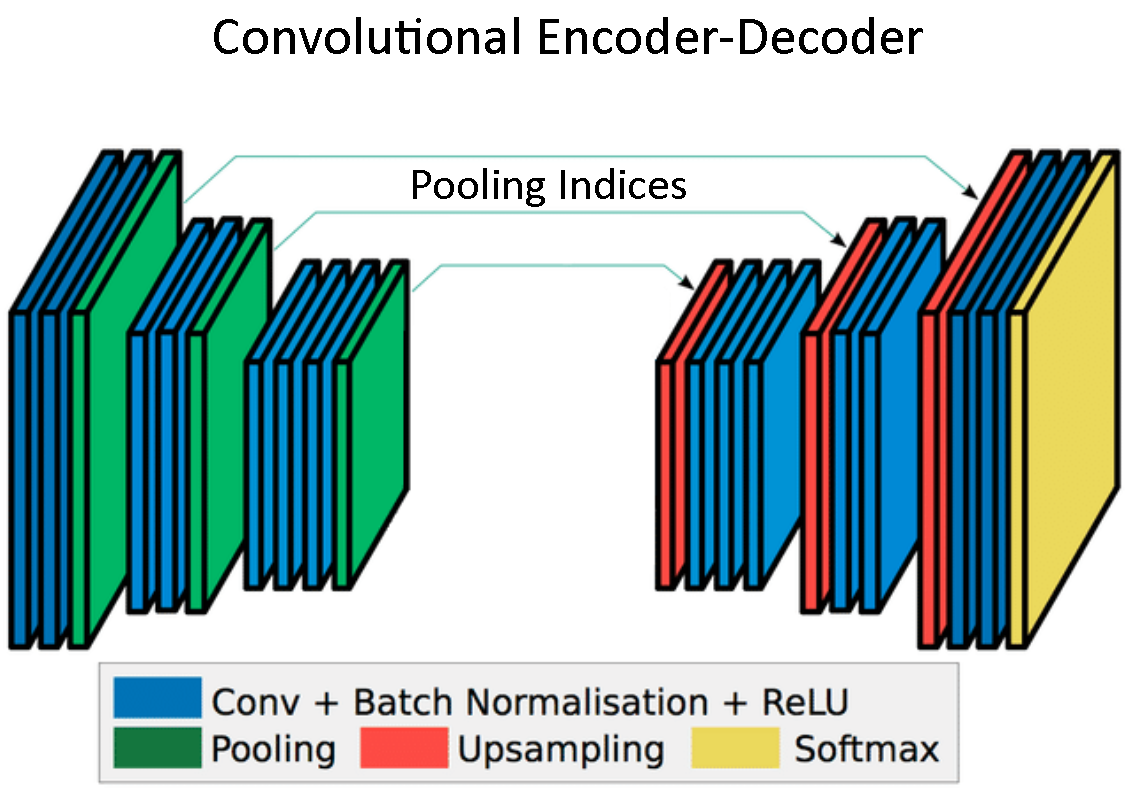
\includegraphics[width=0.8\linewidth]{Structure}
	\caption{}
	\label{fig:Structure}
\end{figure}

%\begin{figure}
%	\centering
%	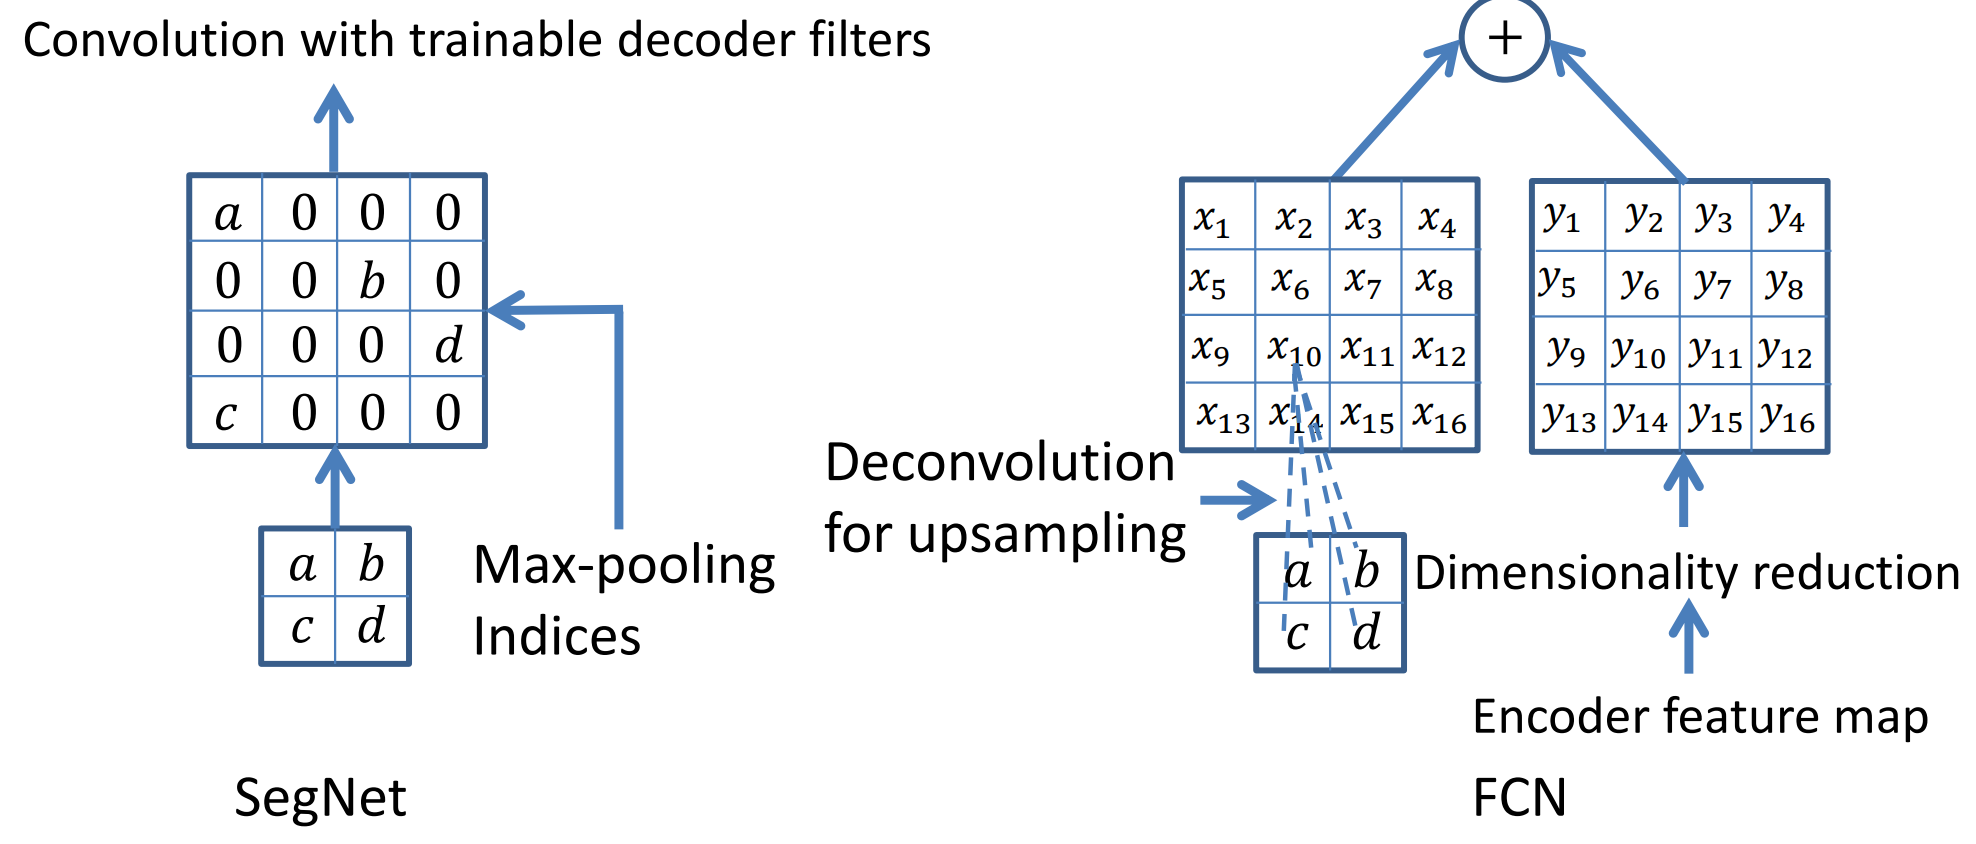
\includegraphics[width=1\linewidth]{MaxPool}
%	\caption{}
%	\label{fig:maxpool}
%\end{figure}

\begin{figure}
	\begin{fadebox}\begin{center}
			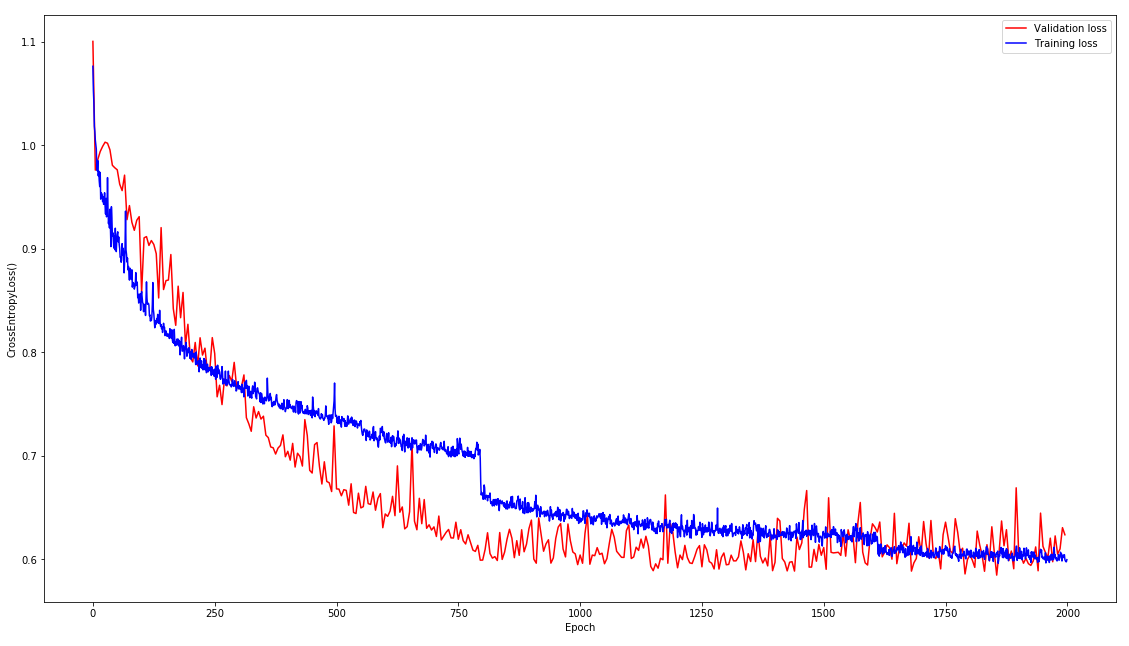
\includegraphics[width=\linewidth,origin=c]{loss}
	\end{center}\end{fadebox}
	\caption{An example caption. Figures can be wrapped in the \texttt{fadebox} 
		environment to provide them with a white background. Note that you have to align the 
		figure again.}\label{fig:example2}
\end{figure}

%% Hvordan regulariseres netværket
%% Data transformeringer 
%% Hyperparametre 

\section{Different Metrics, Different Stories}

%%Tabel med metrics 
%% Gøre vores F1 score fed og skriftstørrelse 100




%Kort beskrivelse af resultater 

\begin{figure}
	\centering
\subfloat{
	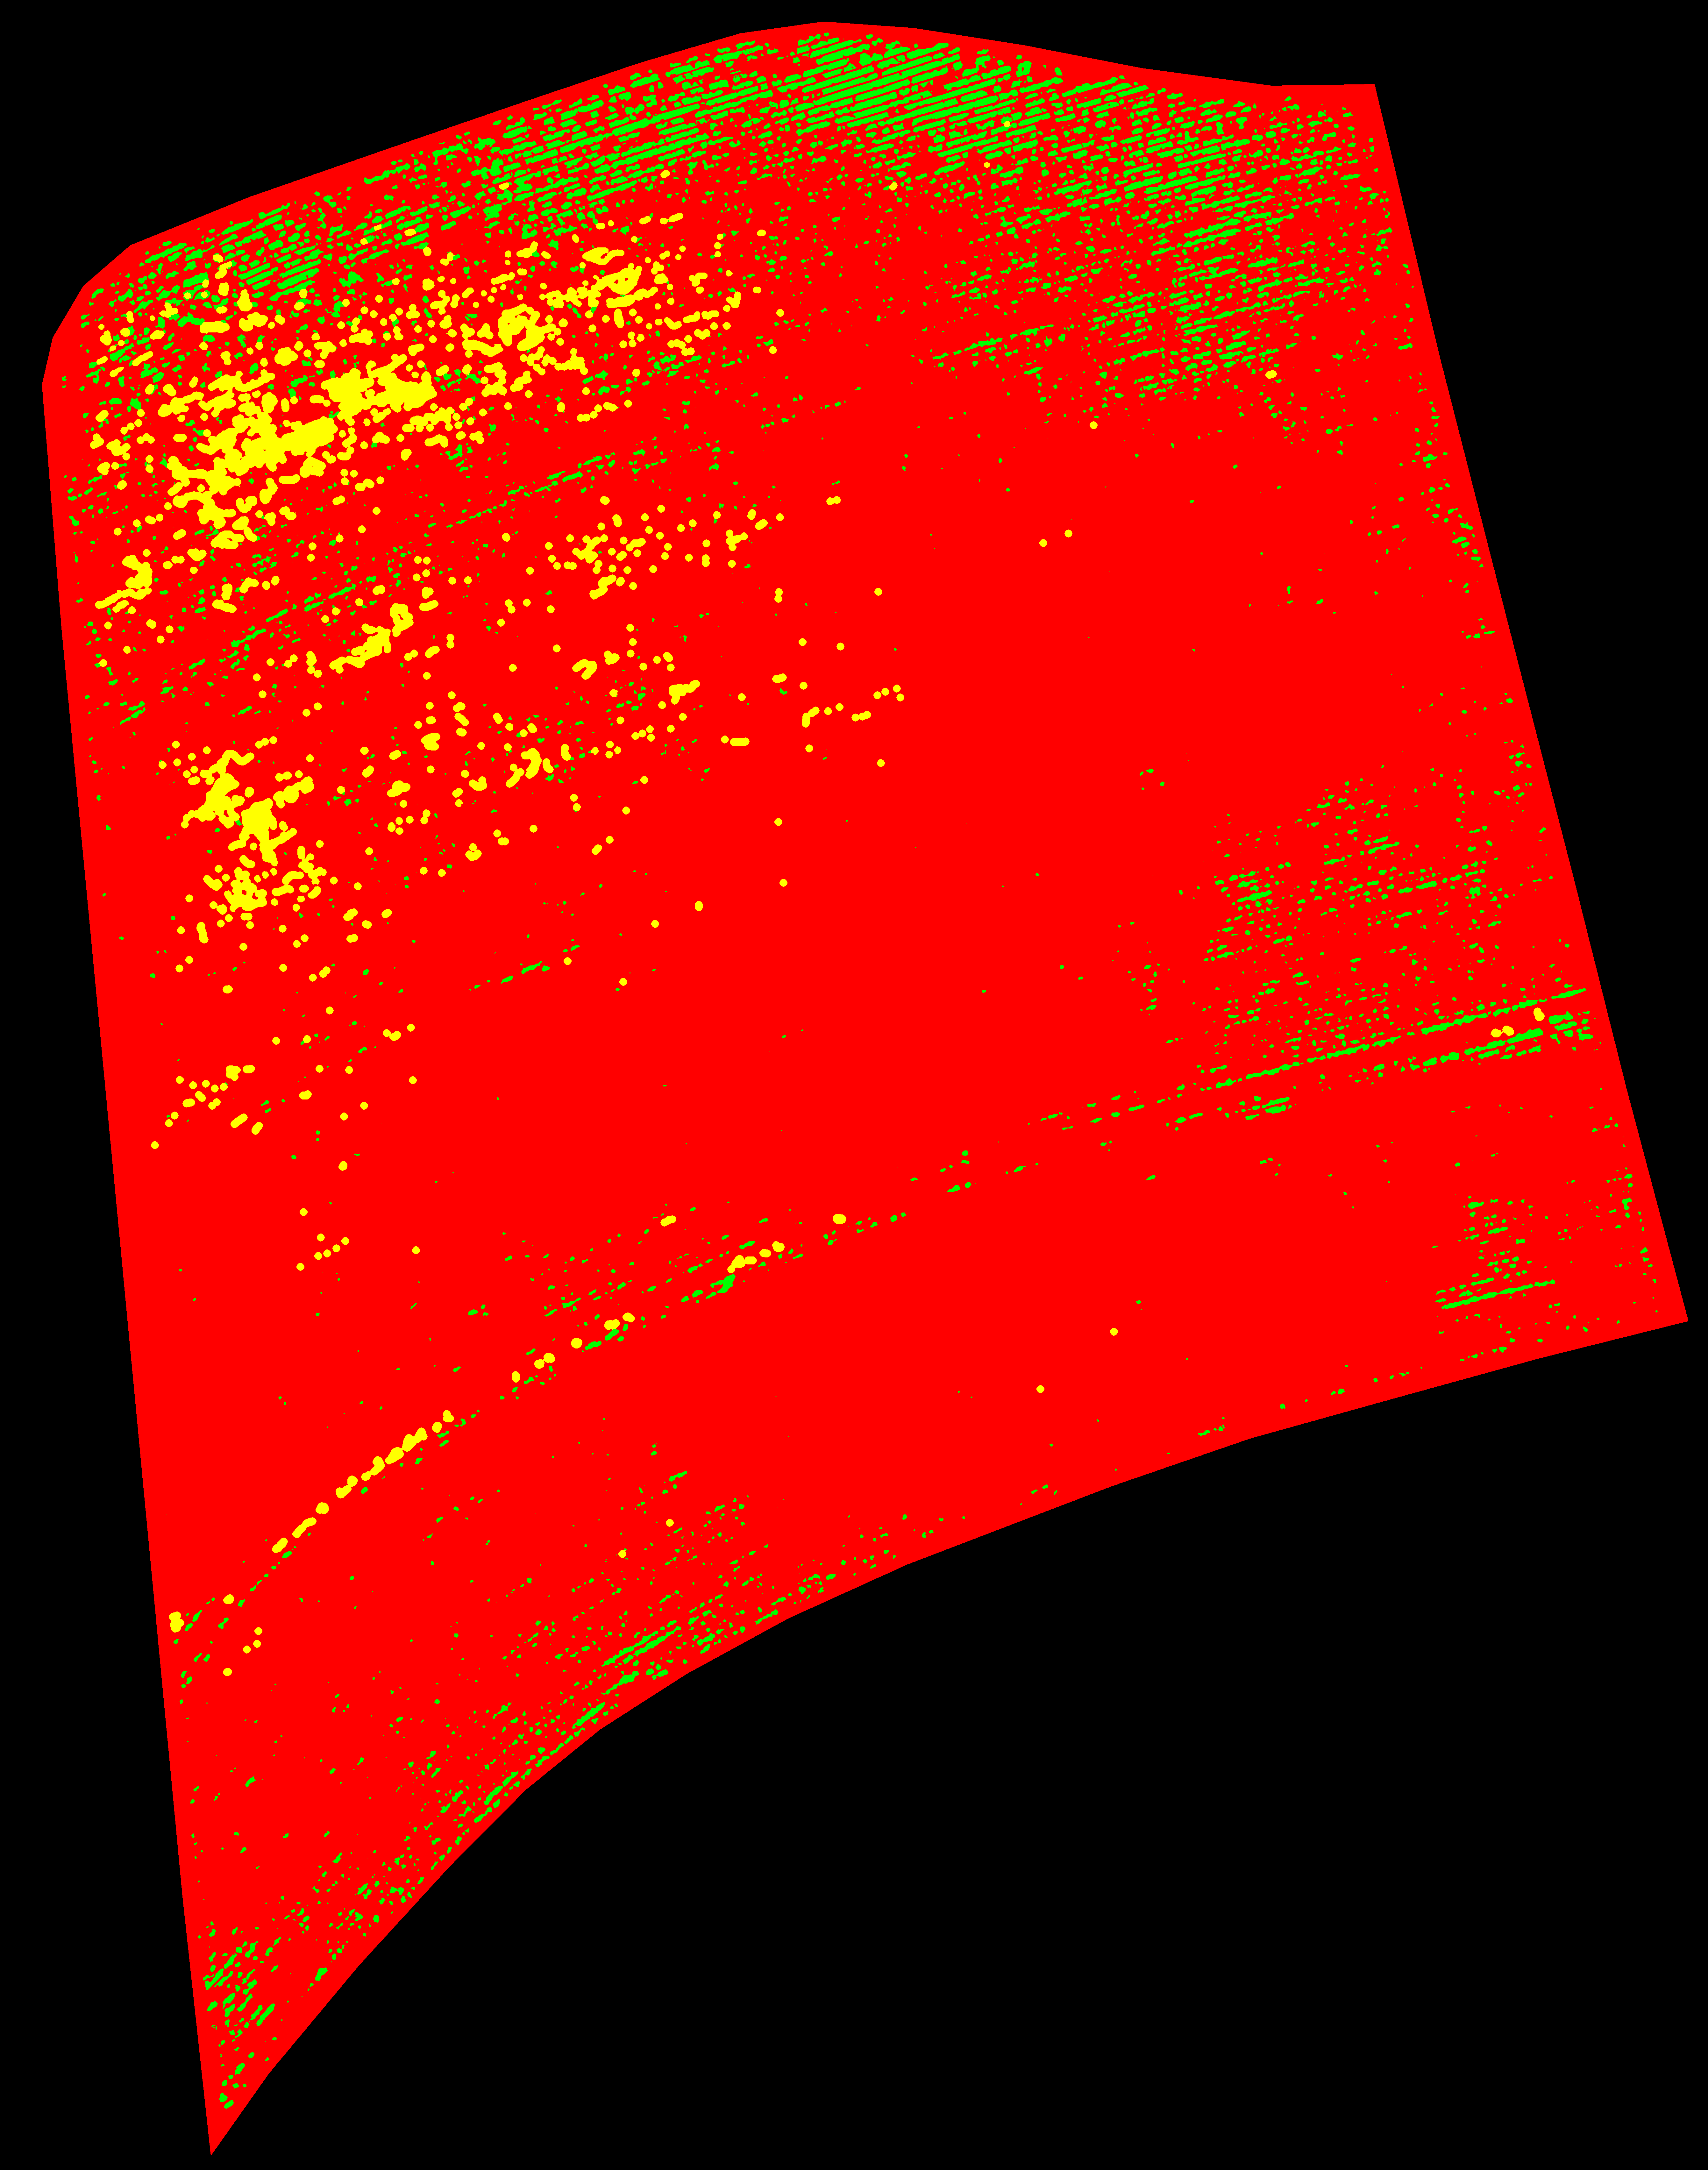
\includegraphics[width=.5\linewidth]{target}	
}
\subfloat{
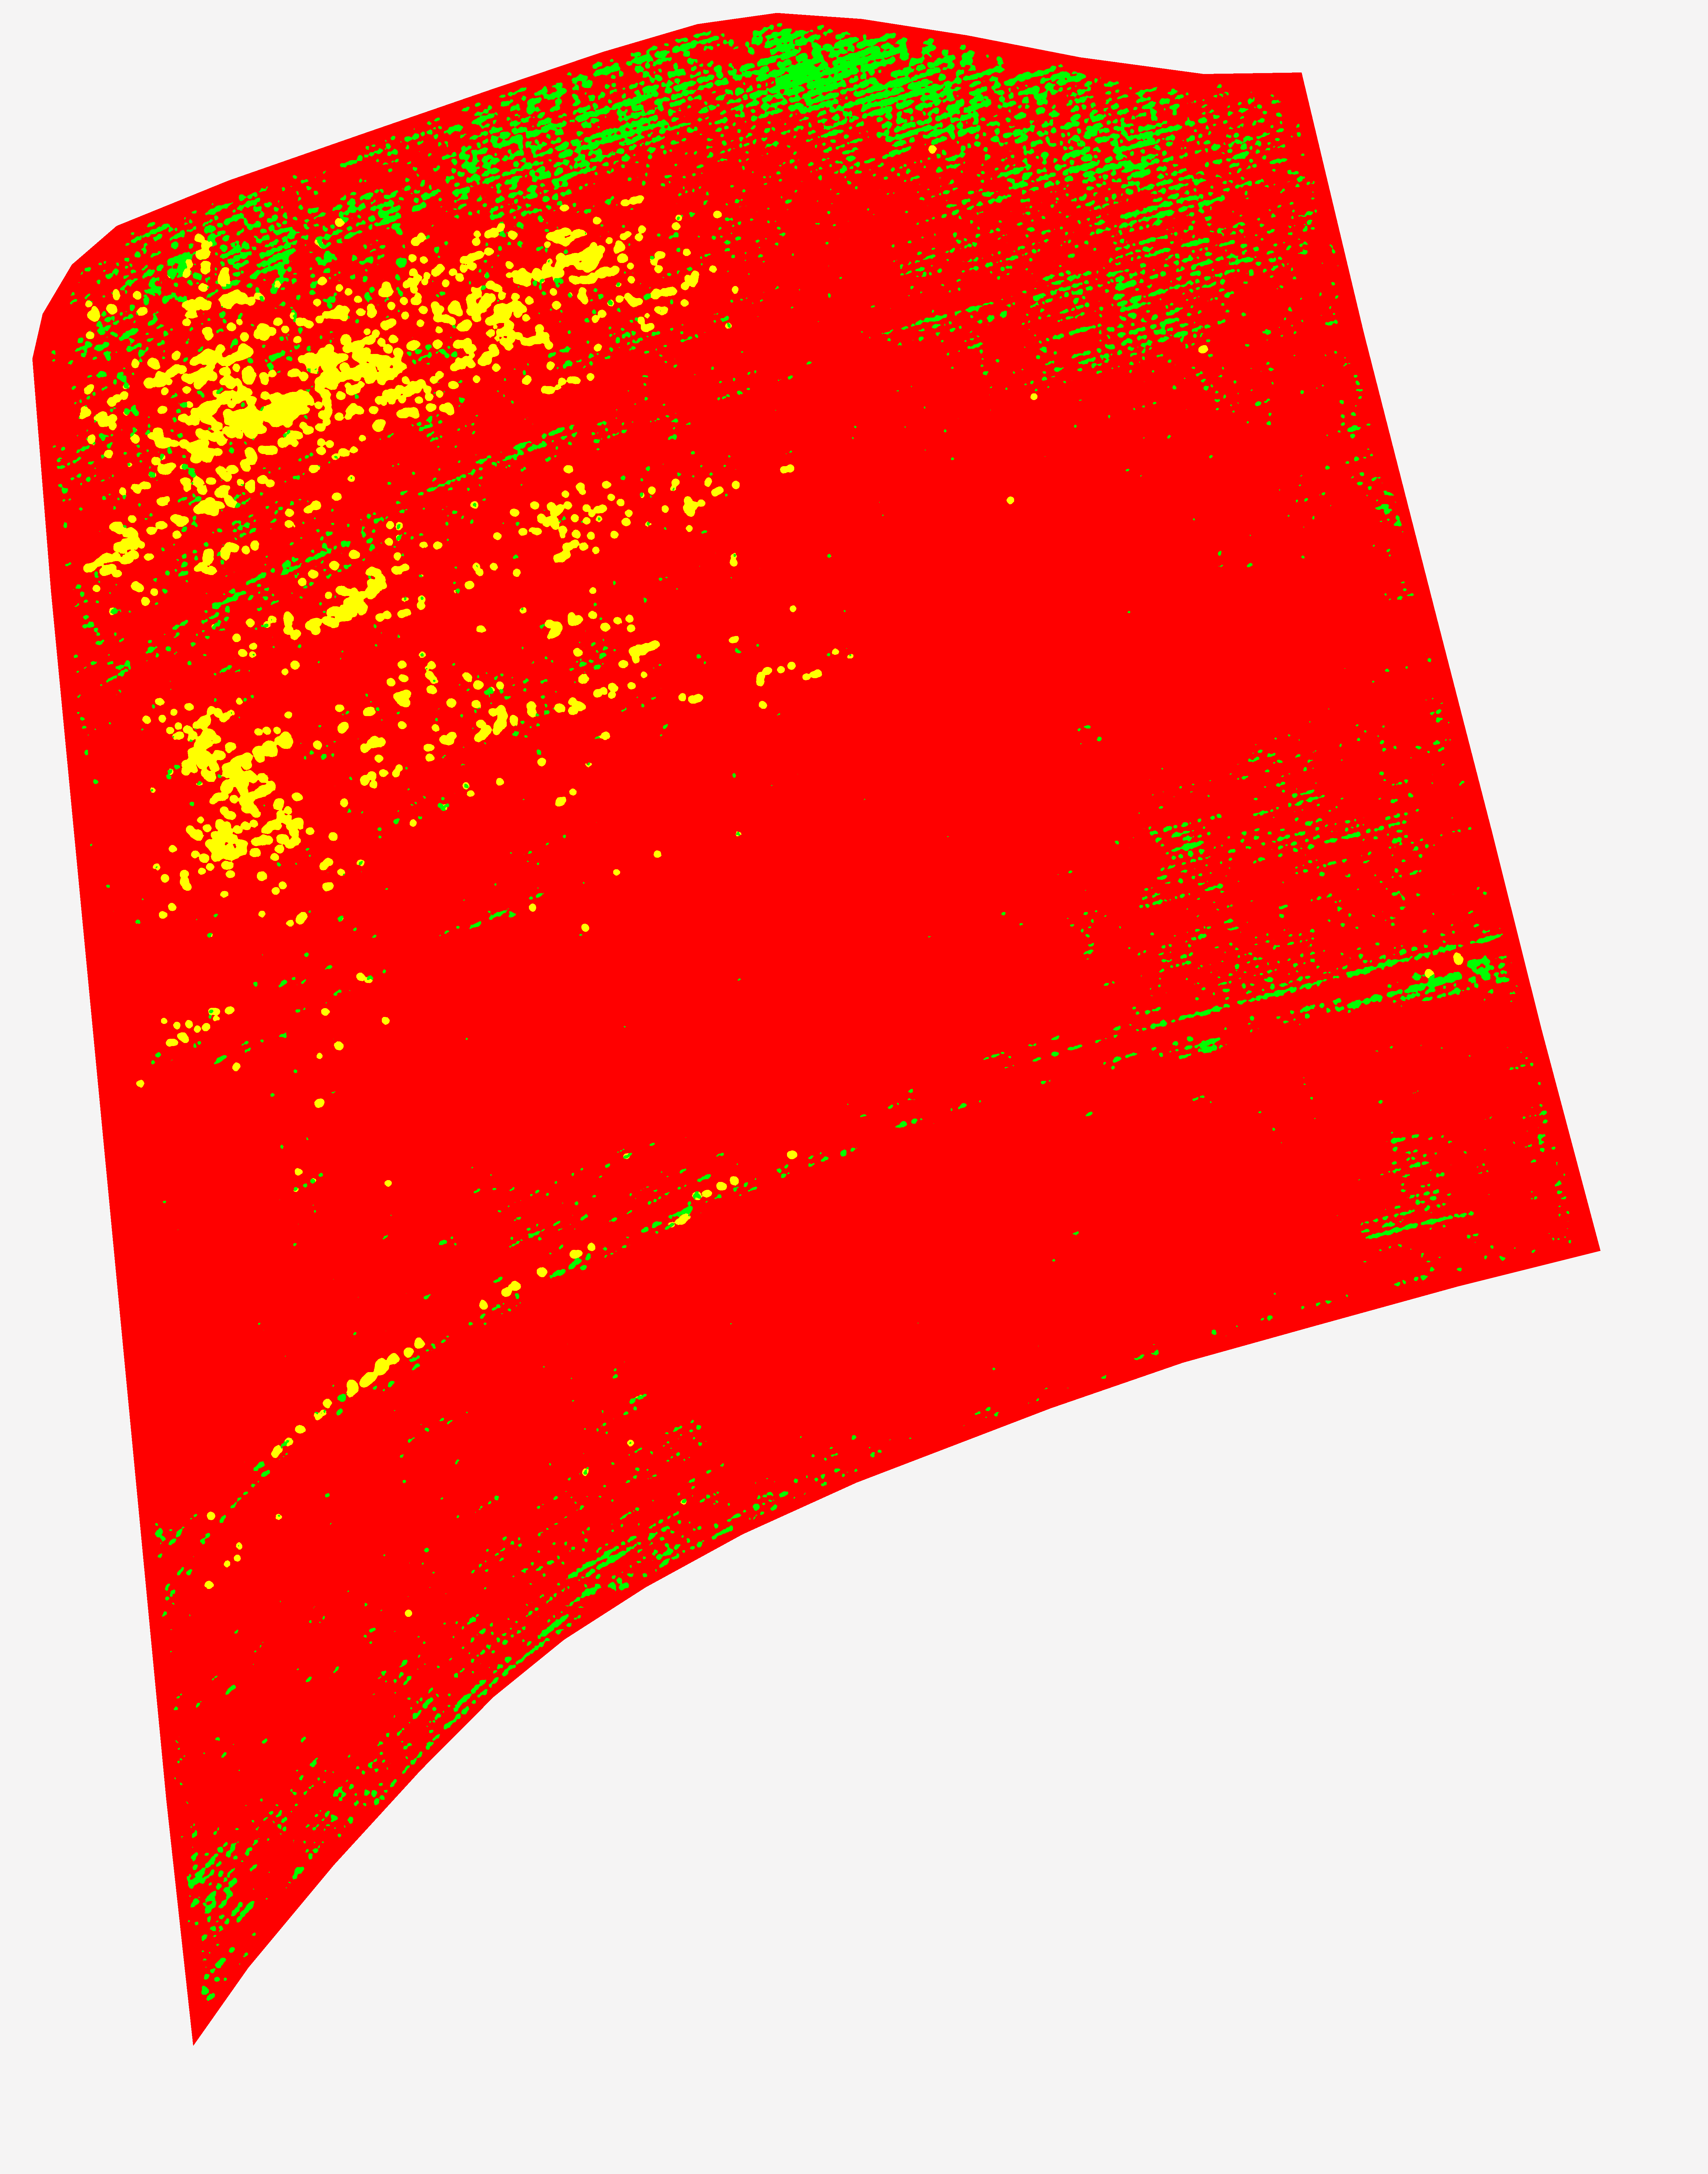
\includegraphics[width=.5\linewidth]{anno}	
}
\caption{An example caption. This figure supports transparency and looks fine on 
the coloured background}\label{fig:example}
\end{figure}

\section{Where Can This Go?}
% Yderligere arbejde
%Perspektiv på problemet 


\end{dtupostercontent}

\end{document}
